%=======================================================================
% LuminaBone — ICRA-format paper (IEEEtran conference mode).
% Metric near-field photometric stereo on bone in confined corridors.
% Compile: pdflatex + bibtex + pdflatex x2. Figures in ./figures/.
%=======================================================================
\documentclass[conference]{IEEEtran}
\IEEEoverridecommandlockouts
\usepackage{amsmath,amssymb,bm}
\usepackage{graphicx}
\usepackage{booktabs}
\usepackage[per-mode=symbol]{siunitx}
\usepackage{algorithm}
\usepackage{algpseudocode}
\usepackage[hidelinks]{hyperref}
\usepackage{cite}

\newcommand{\vn}{\bm{n}}
\newcommand{\vl}{\bm{l}}
\newcommand{\vL}{\bm{L}}
\newcommand{\vg}{\bm{g}}
\newcommand{\vX}{\bm{X}}
\newcommand{\vP}{\bm{P}}
\newcommand{\zt}{\tilde z}

\begin{document}

\title{\LARGE \bf Metric Bone-Surface Reconstruction in Confined Surgical Corridors\\
with a Near-Coaxial Photometric-Stereo Endoscope}

% ICRA 2027 is double-anonymous: submit with the anonymous block below.
% For the camera-ready, swap in the real author block (second, commented).
\author{Anonymous for double-anonymous review\\ Paper ID —}
%\author{Andy Ding$^{1}$%
%\thanks{$^{1}$A.~Ding is with (institution to be completed)
%        {\tt\small andyding09@gmail.com}}%
%}

\maketitle
\thispagestyle{empty}
\pagestyle{empty}

%=======================================================================
\begin{abstract}
Surgery on bone increasingly happens at the end of a narrow access
corridor---a tubular retractor, an arthroscopic portal, an endonasal
approach---where navigation needs the exposed surface in metric
coordinates but the corridor admits no stereo baseline, projector, or
tracked pointer.  The endoscope already inside could supply that surface,
except that a monocular scope has no intrinsic length reference beyond
its own illumination geometry.  We present a near-field
photometric-stereo method for an \SI{18}{\milli\meter} endoscope
carrying four LEDs on a ring of radius \SI{6.05}{\milli\meter}, and show that the
ring baseline suffices to place the surface metrically from a single
pose.  Four lights
overdetermine the three per-pixel unknowns, so the residual of a solve
whose normals are tied to a candidate surface carries geometric
information: minimised over a two-parameter depth family---working
distance and relief gain---it selects the surface placement, with absolute
scale entering through the measured ring radius and the lens
depth-of-field band as prior.  Validated on a CT-instrumented lumbar spine phantom---a demanding
corridor target, with per-vertebra rigid-body structure---the method
reconstructs all three well-conditioned vertebral levels to
\SIrange{2.7}{3.1}{\milli\meter} fiducial RMS under a rigid 6-DOF
alignment, with per-level scale errors of \SIrange{10}{21}{\percent}.
Under the same protocol, classical far-field photometric stereo suffers a
systematic low-frequency bowl (\SI{6.6}{\milli\meter} on its worst well-conditioned level)
and inverse-square shading-to-range fails on every level
(\SIrange{6.4}{9.6}{\milli\meter}); a variant given oracle depth anchoring
bounds the achievable accuracy at \SIrange{1.3}{1.7}{\milli\meter}.
Unmodelled as-built LED geometry biases the recovered working distance by
up to \SI{15}{\milli\meter} and is the dominant remaining error; the
two failing levels are traced to a three-fiducial degeneracy and a
confidence-mask collapse.
\end{abstract}

%=======================================================================
\section{INTRODUCTION}

% ---- Fig. 1: top of page 1 ----
\begin{figure}[!t]
\centering
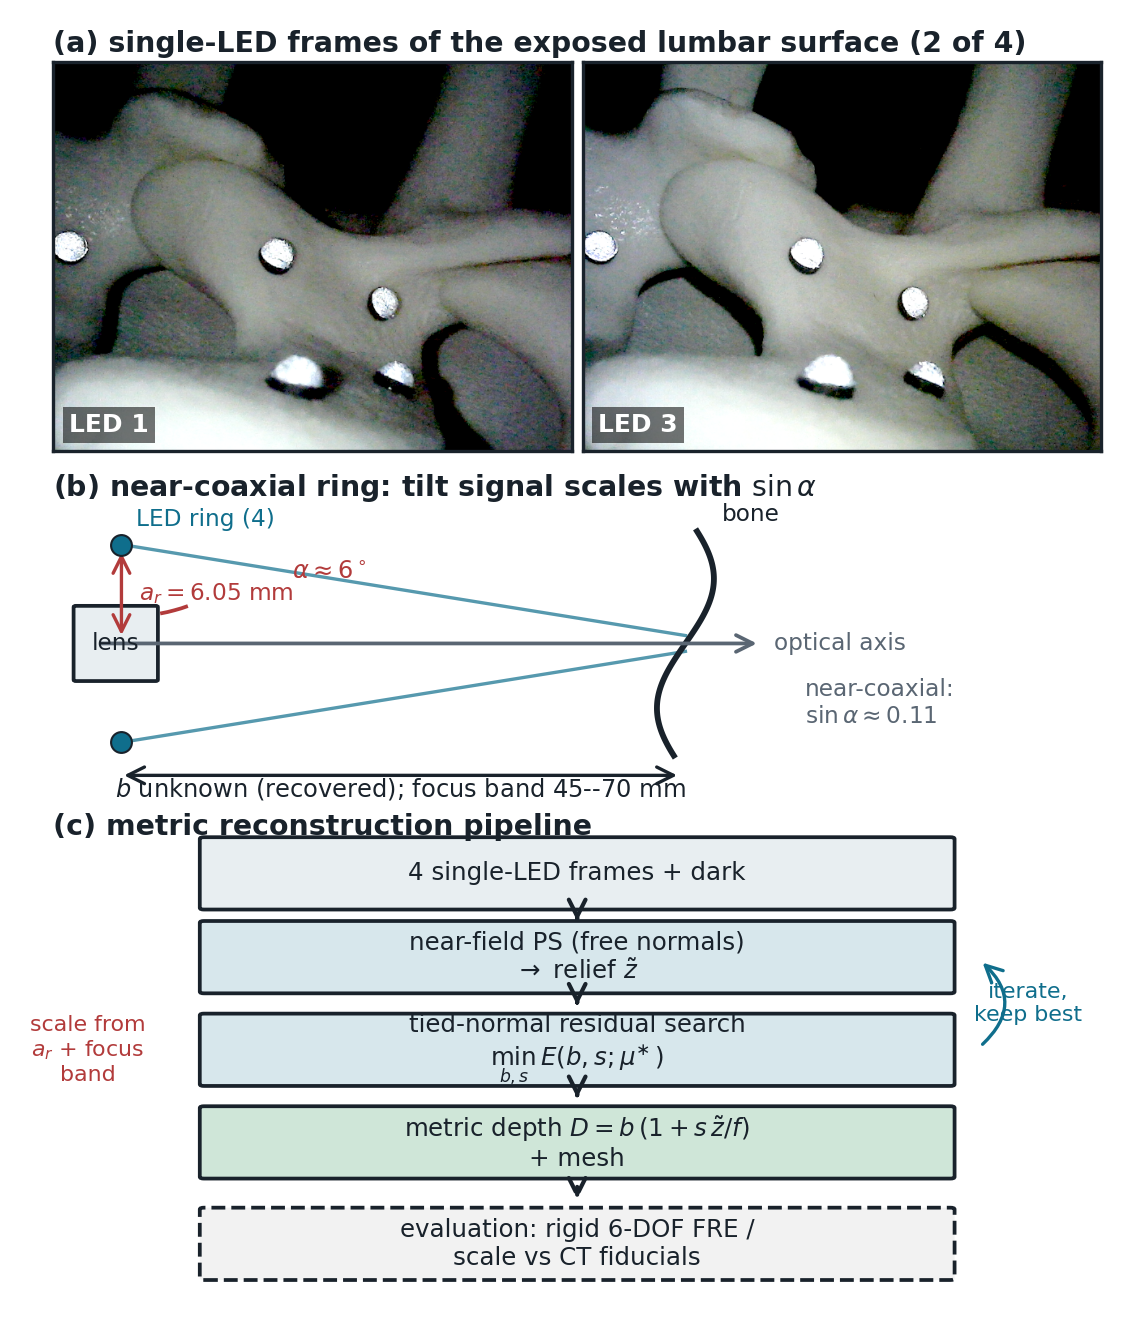
\includegraphics[width=0.98\columnwidth]{figures/fig1_pipeline.png}
\caption{\textbf{System overview.} (a)~Two of the four single-LED frames
of an exposed lumbar segment; the shading change between opposing LEDs
encodes surface tilt, and the specular dots are the evaluation fiducials.
(b)~The LEDs sit on a ring of radius $a_r=\SI{6.05}{\milli\meter}$, only
$\alpha\approx\ang{6}$ off-axis at the working distance: near-field and
near-coaxial.  (c)~Pipeline: a free-normal near-field solve proposes
relief~$\zt$; a tied-normal residual search recovers working distance~$b$
and relief gain~$s$, with metric scale entering through $a_r$; the
reconstruction is scored against CT fiducials (dashed).}
\label{fig:system}
\end{figure}

% ---- Clinical context & hook (1 short paragraph) ----
\IEEEPARstart{B}{one}-directed surgery is migrating into narrow access
corridors: tubular retractors in the spine~\cite{foley2003}, arthroscopic
portals in joints, endoscopic approaches to the skull base.  Navigation
against preoperative imaging then hinges on registering the exposed bone
surface---in the spine, per vertebra, since the column flexes at the
discs~\cite{herring1998}.  Whether guidance is manual or
robotic~\cite{shoham2003bonemounted}, that registration currently costs
either intraoperative 3-D imaging (cone-beam CT / O-arm, with added
radiation and workflow interruption~\cite{mendelsohn2016}) or tracked
instruments that demand line of sight into a corridor that barely admits
the scope.  Yet the endoscope is already looking at the bone; if it could
measure that surface \emph{metrically} on its own, the surface itself
could drive registration with no added radiation or tracking hardware.

% ---- Technical gap & prior art (1--2 paragraphs) ----
Metric shape from the scope already in the wound is, however, exactly
where existing pipelines fall short~\cite{maierhein2013optical}.
Multi-view geometry---structure-from-motion, SLAM, and their learned
variants~\cite{ozyoruk2021endoslam}, engineered for intra-articular
reconstruction in Dense-ArthroSLAM~\cite{marmol2019densearthroslam}---needs texture and
parallax that wet, low-texture bone provides poorly, and monocular
reconstruction is in any case scale-blind without an external
reference.  Photometric
stereo~\cite{woodham1980} fits the setting better: it recovers a dense
normal field from a fixed viewpoint under varying illumination and is
albedo-invariant, which matters on stained, textured bone.  It has been
demonstrated through endoscopes on soft
tissue~\cite{parot2013photometric,collins2012close,hao2020capsule}, but with
accuracy unreported, mapped only per pixel, or confined to a bench
target (Sec.~\ref{sec:related}); none is evaluated against tomographic
ground truth.
Near-field formulations with per-pixel light directions and inverse-square
attenuation are well
understood~\cite{queau2018led,batlle2022photometric,mecca2014near}, yet
they obtain absolute scale from outside the images---a known or tracked
working distance, or a calibrated auxiliary sensor.  The scale, in
principle, is already in the illumination: the decline of the scope's own
light encodes range, and recent work recovers metric depth from
it~\cite{rodriguezpuigvert2023lightdepth,batlle2023lightneus,iranzo2025endometric}.
But that line has been developed for single co-located sources with
light--camera baselines of ${\sim}\SI{3}{\milli\meter}$ or smaller, on
deformable gastrointestinal tissue, and its accuracy has not been tested against the
millimetre demands of surgical navigation on rigid anatomy.

The obstacle specific to a small bone-facing scope is geometric.  A ring
of LEDs around the objective is \emph{near-coaxial}: at
$b\approx\SI{55}{\milli\meter}$ each light is only $\alpha\approx\ang{6}$
off-axis, so the tilt-encoding lateral component of every light vector
scales with $\sin\alpha\approx0.11$, the conditioning of the four-light
system degrades as $\sqrt{2}\cot\alpha$, and a far-field model integrates
its mis-fit into a low-frequency bowl that no global scale or offset can
remove.  Errors in the assumed light geometry are amplified by the same
factor, so the wiring, aim, and emission profile of the LEDs must be
identified rather than assumed.

% ---- Proposed solution (1 paragraph) ----
This paper presents a metric near-field photometric-stereo pipeline for
that regime (Fig.~\ref{fig:system}).  A free-normal near-field solve
proposes a relative relief map; the reconstruction then searches a
two-parameter metric depth family---working distance $b$ and relief gain
$s$---by minimising the four-image photometric residual of the candidate
surface with normals \emph{tied} to it, so that a wrong geometry produces
a shading misfit the per-pixel solve cannot absorb.  Because four lights
overdetermine the three per-pixel unknowns---the classical virtue of
four-source photometric stereo~\cite{coleman1982,barsky2003}---this
residual is informative, and because the ring radius $a_r$ is a measured
hardware length, its minimum selects an absolute scale; the only prior is
the lens depth-of-field band, a bench property of the fixed-focus optics.
The rig itself is identified in situ: the LED wiring by a
permutation study against the fiducial depths of two levels, the beam aim
by a centroid analysis, and the emission exponent by an end-to-end
sensitivity study.

% ---- Contributions (3 bullets) ----
The contributions are:
\begin{itemize}
\item a metric formulation of near-field photometric stereo for
near-coaxial ring illumination: a tied-normal residual objective over a
two-parameter depth family whose absolute scale comes from the LED ring
baseline, optimised by a multi-start, keep-best search inside a
bench-measured focus band (Sec.~\ref{sec:metric});
\item in-situ identification of a ring-lit endoscope:
index$\to$azimuth wiring by a 24-permutation study
($r={+}0.97/{+}0.99$ vs.\ ${-}0.97/{-}0.99$ for the diametric flip), a
beam-centroid analysis that separates LED \emph{aim} from LED
\emph{position} and reveals convergent aim on this rig, and a sensitivity
study showing that the photometric residual under-constrains the emission
exponent while final accuracy depends on it strongly
(Secs.~\ref{sec:rig},~\ref{sub:mu});
\item a fiducial-based evaluation on a CT-instrumented lumbar phantom
across five vertebral levels---rigid-only 6-DOF FRE of
\SIrange{2.7}{3.1}{\milli\meter} on the three well-conditioned levels,
registration-free scale checks, ablations against far-field,
inverse-square, and oracle-anchored variants, and an analysis of both
failure cases (Sec.~\ref{sec:exp}).
\end{itemize}

%=======================================================================
\section{RELATED WORK}\label{sec:related}

\subsection{Photometric Stereo and Near-Field Illumination}
Woodham's formulation~\cite{woodham1980} recovers per-pixel normals from
$\ge$3 distant illuminations, integrated to depth by, classically, the
Frankot--Chellappa projection~\cite{frankot1988}; four sources add the
redundancy needed to reject highlights and
shadows~\cite{coleman1982,barsky2003}.  Non-Lambertian extensions
(robust, parametric, example-based, learned) attack the reflectance term
but retain far-field lights~\cite{shi2019benchmark}, under which shape is
recoverable only up to the generalised bas-relief
ambiguity~\cite{belhumeur1999basrelief}.  Near-field sources change both
statements: Qu\'eau~et~al.~\cite{queau2018led} give the complete LED
forward model---position, principal direction, $\cos^\mu$ anisotropy,
inverse-square fall-off---with calibration and solvers, the attenuation
term makes near-source shape-from-shading
well-posed~\cite{prados2005}, and the LUCES benchmark quantifies both the
necessity and the ceiling of the model: a naive far-field method degrades
to \ang{37.5} mean normal error at 10--30 cm, while the best calibrated
near-field solvers, given 52 individually calibrated LEDs, average
\ang{13.3} normal and \SI{3.2}{\milli\meter} depth
error~\cite{mecca2021luces}.
Semi-calibrated variants estimate light intensities in the
solve~\cite{queau2017semicalibrated}, uncalibrated near-light
photometric stereo has been analysed in~\cite{papadhimitri2014uncalibrated},
and dedicated procedures calibrate point-light
positions~\cite{ma2023robust}.  All of this work estimates normals (or
depth up to the modelled lights) with the working distance essentially
known; the present paper inverts the emphasis and estimates the metric
surface placement itself, using the ring baseline as the length
reference.

\subsection{Endoscopic Reconstruction and Metric Scale}
That an endoscope's illumination geometry is special was recognised
early: Okatani and Deguchi~\cite{okatani1997shape} solved shape-from-shading
with the source at the projection centre, the limiting case our
\ang{6}-off-axis ring sits just beyond.  Photometric stereo endoscopy was
introduced by Parot~et~al.~\cite{parot2013photometric} on phantoms and
\emph{ex vivo} human gastrointestinal tissue, and engineered into a
\SI{14}{\milli\meter} clinical gastroscope used in vivo in eight human
rectums~\cite{durr2014system}---but the technique is, by its authors'
own description, qualitative in height: low-frequency shape is discarded
by a high-pass filter, and across the programme no surface-accuracy
figure was reported.  Close-range colour-multiplexed PS in
laparoscopy~\cite{collins2012close} computes absolute depth from a
calibrated attenuating light model, but reports only per-pixel error maps
spanning \SIrange{1}{6}{\milli\meter} ex vivo at ${\sim}35$ mm range,
with no summary statistic; capsule PS with four LEDs at
\SI{5.5}{\milli\meter} offset~\cite{hao2020capsule} reaches
\SI{0.51}{\milli\meter} RMSE, but at \SI{21}{\milli\meter} working
distance (a baseline-to-depth ratio $2.3\times$ ours), on a single
smooth convex target, with the metric seed taken from a specular
highlight whose millimetre-level error triples the surface error.
Batlle~et~al.~\cite{batlle2022photometric} photometrically calibrate a
clinical colonoscope to three grey levels and reconstruct single-view
colon surfaces at \SI{7}{\percent} (\SI{2.8}{\milli\meter}) mean depth
error---in simulation; their in-vivo reconstruction has arbitrary scale,
since absolute scale there requires known albedo and camera auto-gain.
The illumination-decline line inherits the same ambiguity:
LightDepth~\cite{rodriguezpuigvert2023lightdepth} reports
\SIrange{3.7}{4.4}{\milli\meter} MAE on the C3VD colon phantom
\emph{after median alignment to ground-truth scale};
LightNeuS~\cite{batlle2023lightneus} reaches \SI{2.80}{\milli\meter} MAE
with twenty views and ground-truth-registered metric poses, degrading to
\SI{8.23}{\milli\meter} when camera motion falls below
\SI{1}{\centi\meter}; and EndoMetric~\cite{iranzo2025endometric} recovers
true metric scale from a ${\sim}\SI{3}{\milli\meter}$ light--camera
baseline, at ${\sim}\SI{1}{\percent}$ scale error within \SI{8}{\milli\meter}
of the mucosa but \SI{5}{\percent} by \SI{20}{\milli\meter} (in
simulation), its observability decaying with the baseline-to-distance
ratio.  The present
work pushes the same physics to a harder operating point and a stronger
evaluation: a \SI{6.05}{\milli\meter} baseline at \SI{55}{\milli\meter}
(ratio $0.11$), four sequenced lights that overdetermine the per-pixel
solve in place of learning or constant-albedo assumptions, and rigid,
textured bone scored against CT fiducials rather than simulation or
scale-aligned metrics.

\subsection{Surgical Surface Reconstruction and Registration}
The accuracy bar for bone-surface registration is set by systems with
far more favourable sensing geometry, with the spine---the target of our
evaluation---the most quantified case.  A tracked stylus sampling ${\sim}20$ lamina
points registers a dry-bone lumbar phantom to
$0.96\pm\SI{0.24}{\milli\meter}$ RMS~\cite{tamura2005}; structured-light
optical topographic imaging acquires ${>}250$k points and registers in
${\sim}5$ s, with clinical pedicle-screw errors of
${\sim}\SI{1.2}{\milli\meter}$ median~\cite{jakubovic2018}; stereovision
serves the same role in open exposures~\cite{ji2015}, with surface-based
spine registration analysed as early as
Herring~et~al.~\cite{herring1998}, and accuracy reported as fiducial and
target registration error after
Fitzpatrick~et~al.~\cite{fitzpatrick1998}.  Deployed 3-D navigation
delivers 1.2--1.75 mm mean translational accuracy in
vivo~\cite{guha2017}---but these are open-field or line-of-sight systems,
and their static figures erode in use: vertebral displacement from
surgical manipulation averages \SI{1.6}{\milli\meter}, respiration displaces
vertebrae by \SI{2.0}{\milli\meter} on average (most in the lower
thoracic spine), and error grows by
${\ge}\SI{4}{\milli\meter}$ five levels from the reference
frame~\cite{guha2019}.  Rigid alignments come from point
correspondences~\cite{kabsch1976,umeyama1991} or ICP~\cite{besl1992};
shape-from-shading has been registered to CT in bronchoscopy via
pq-space~\cite{deligianni2003pq}, and robotic spine systems have explored
ultrasound as the registration modality~\cite{li2024ultrasound}.  Each of
these opens the field to a projector or stereo head, adds a transducer,
or relies on tracked hardware; we keep the single near-coaxial scope
already in the corridor and move the difficulty into the photometric
solve.  Consistent with surgical practice, every vertebra is treated as
its own rigid body~\cite{herring1998}.

%=======================================================================
\section{HARDWARE AND EXPERIMENTAL SETUP}\label{sec:rig}

\subsection{Probe Hardware}\label{sub:hw}
The probe is an \SI{18}{\milli\meter}-OD rigid endoscope---the diameter
class of tubular-retractor MIS access~\cite{foley2003}---with a monocular
camera (native $640\times480$, diagonal field of view
$\le\ang{90}$) in a central $\varnothing\SI{9.7}{\milli\meter}$ bore and
four white LEDs in tip pockets at azimuths \ang{0}, \ang{90}, \ang{180},
\ang{270} around the lens.  The CAD pocket-centre radius is
\SI{5.09}{\milli\meter}; the as-built emitter radius, measured with
calipers, is $a_r=\SI{6.05}{\milli\meter}$, and the measured value is what
enters the model.  The emitters additionally exhibit a
${\sim}\SI{2}{\milli\meter}$ axial spread along the probe axis, an
as-built deviation that the ideal-ring model of Sec.~\ref{sec:metric}
does not capture and to which the error analysis returns.  The LEDs are
sequenced one at a time under constant-current DC drive (PWM dimming
beats against the rolling shutter and masquerades as shading), with
exposure and gain locked for the whole session.

\subsection{Phantom, Fiducials, and Capture Protocol}\label{sub:phantom}
The target is a rigid lumbar phantom (Sawbones 1324-56, L1--sacrum, solid
foam), unmodified, instrumented with four retroreflective spherical
fiducials per vertebra (level~7: three usable) and CT-scanned with the
fiducials in place.  Each fiducial is visible both in CT (a surface
crater) and in the images (a specular dot), providing the 2-D/3-D
correspondences that serve as ground truth for evaluation.  Each capture
records a dark frame plus four single-LED frames from a fixed pose,
flushing the camera's frame buffer after every LED switch so the four
images cannot be misassigned.

\subsection{Calibration and Radiometric Preprocessing}\label{sub:sys}
Intrinsics and distortion come from a ChArUco calibration (121 views,
\SI{0.11}{px} reprojection); the working focal length
$f\!\approx\!\SI{860}{px}$ is additionally validated by four-point PnP
reprojection (\SI{0.42}{px} residual) using SQPnP~\cite{terzakis2020}.
The photometric solve treats the mildly distorted pixel grid as pinhole;
the distortion model is applied when projecting for pose validation.
Frames are converted to linear luminance in four steps: dark subtraction,
sRGB$\to$linear decoding, Rec.\,601 luminance, and specular inpainting of
bright low-saturation pixels (the retroreflective fiducials violate
Lambert).  Because frames are captured sequentially, each is divided by
its median to cancel per-frame exposure drift---a spatially constant
correction that leaves the shading field intact; the residual per-LED
power difference is absorbed by per-LED gains estimated inside the
objective (Sec.~\ref{sub:objective}).

\subsection{Near-Coaxial Conditioning}\label{sub:cond}
At working distance $b$ each LED subtends
$\alpha=\arctan(a_r/b)\approx\ang{6}$, so a far-field light direction is
$\vL_s=[\sin\alpha\cos\phi_s,\ \sin\alpha\sin\phi_s,\ \cos\alpha]^\top$.
Stacking the four ring azimuths, $\bm L^\top\bm L=
\mathrm{diag}(2\sin^2\alpha,\,2\sin^2\alpha,\,4\cos^2\alpha)$, so the
condition number of the light matrix is exactly $\sqrt{2}\cot\alpha\approx
\sqrt{2}\,b/a_r$ ($\approx\!13$ at \SI{55}{\milli\meter}): image noise is
amplified into the tangential normal components by $\sim\!1/\sin\alpha$,
recovered relief is compressed, and errors in the assumed light geometry
are magnified by the same factor.  This is the regime the method is
designed for.

\subsection{Wiring and Aim Identification}\label{sub:wiring}
The map from frame index to ring azimuth must be established before any
reconstruction.  Scoring all $4!$ assignments by the correlation between
reconstructed depth at the fiducials and the fiducial depths of two
levels identifies the physical wiring (LED1$\to$\ang{90},
LED2$\to$\ang{270}, LED3$\to$\ang{180}, LED4$\to$\ang{0}) at
$r=+0.97/+0.99$, while the diametrically flipped labelling \emph{inverts}
the surface ($r=-0.97/-0.99$): a mislabelling is not a perturbation but a
sign flip of the recovered geometry, a silent failure mode for any
multi-LED rig.  An independent cue corroborates the assignment: dividing
each single-LED image by the four-LED mean cancels albedo and shape, and
the brightness-weighted centroid of the ratio image marks where that
LED's \emph{beam} lands.  Unanimously across all five captures, the
vertical pair's beams land on the side opposite their ring positions:
those LEDs are aimed convergently, crossing the optical axis before the
working distance.  Beam aim redistributes intensity but cannot flip the
side light arrives from, so incidence---and hence the wiring---is set by
LED position; the aim finding instead shows that a parallel-aim emission
model is only an approximation on this rig (Sec.~\ref{sub:mu}).  A
one-time bench check (powering each LED individually)
would confirm the assignment directly.

%=======================================================================
\section{METRIC NEAR-FIELD RECONSTRUCTION}\label{sec:metric}

\subsection{Near-Field Model and Free-Normal Solve}\label{sub:nf}
In the camera frame ($+x$ right, $+y$ up, $+z$ toward the camera) a pixel
$(u,v)$ at depth $D$ back-projects to
$\vX=D\,[\,(u-c_x)/f_x,\ -(v-c_y)/f_y,\ -1\,]^\top$, and LED $s$ sits at
$\vP_s=[a_r\cos\phi_s,\ a_r\sin\phi_s,\ 0]^\top$.  With incident direction
$\vl_s=(\vP_s-\vX)/\lVert\vP_s-\vX\rVert$ and attenuation
\begin{equation}
w_s=\frac{\cos^{\mu}\theta_s}{\lVert\vP_s-\vX\rVert^{2}},\qquad
\cos\theta_s=\frac{D}{\lVert\vP_s-\vX\rVert},
\label{eq:att}
\end{equation}
the point-source model $I_s=\rho\,(\vn\!\cdot\!\vl_s)\,w_s$---with the
$\cos^\mu$ emitter anisotropy standard for LEDs~\cite{moreno2008}, aimed
along the optical axis---linearises by moving the attenuation to the
observation,
$m_s:=I_s/w_s=\vg\!\cdot\!\vl_s$ with $\vg=\rho\vn$, giving a per-pixel
$4\times3$ least-squares system
\begin{equation}
\hat\vg=(\bm\Lambda^{\!\top}\bm\Lambda+\epsilon\bm I)^{-1}
\bm\Lambda^{\!\top}\bm m,\qquad
\bm\Lambda=[\vl_1\ \vl_2\ \vl_3\ \vl_4]^{\!\top}.
\label{eq:solve}
\end{equation}
The normals $\hat\vg/\lVert\hat\vg\rVert$ are integrated by
Frankot--Chellappa~\cite{frankot1988} (even reflection, zero DC) into a
\emph{relative} relief $\zt(u,v)$, median-centred (a 1--99-percentile
clip is applied only to the downsampled copy used inside the search
objective; the full-resolution relief that forms the returned surface is
unclipped).  Since $\bm\Lambda$ and $w_s$ depend on $D$, the solve is
iterated with the current depth estimate.  Up to here the pipeline is
standard near-field photometric stereo; the question is what metric depth
to attach to $\zt$.

\subsection{A Two-Parameter Metric Depth Family}\label{sub:family}
We parameterise the metric surface by a working distance $b$ (mm) and a
dimensionless relief gain $s$,
\begin{equation}
D_{b,s}(u,v)=b\Bigl(1+s\,\frac{\zt(u,v)}{f}\Bigr),
\label{eq:family}
\end{equation}
where dividing by the focal length $f$ of the grid over which $\zt$ was
integrated makes the family resolution-invariant and puts $s$ on a
natural scale: $s=1$ is the perspective-consistent gain, so $s$ reads out
directly how much the near-coaxial solve compresses or inflates relief.
Under far-field lighting a family like \eqref{eq:family} would be
unobservable---relief gain is the flattening direction of the generalised
bas-relief ambiguity~\cite{belhumeur1999basrelief}---and it is exactly
the near-field terms that break it~\cite{papadhimitri2014uncalibrated}.
$(b,s)$ are also precisely the two degrees of freedom that anchored
near-field pipelines take from an external depth reference; here they are
estimated from the images.

\subsection{The Tied-Normal Photometric Objective}\label{sub:objective}
With four lights and three per-pixel unknowns, \eqref{eq:solve} is
overdetermined, so a residual survives any inconsistency between the four
images and the assumed geometry.  Where the normals in that residual come
from is decisive.  Solved freely per pixel, they tilt to compensate a
wrong $(b,s)$ and the objective goes flat.  Candidates are therefore
evaluated with normals \emph{tied} to the surface: from $D_{b,s}$ we form
the 3-D point map $\vX(u,v)$, take finite-difference tangents
$\partial_u\vX,\partial_v\vX$, and set
$\vn=\pm\,\partial_u\vX\times\partial_v\vX$ oriented toward the camera.
The model shading is $\hat m_s=(\vn\!\cdot\!\vl_s)\,w_s$ clamped at zero,
and the only remaining freedoms are physically nuisance ones: a per-pixel
albedo $\rho$, one gain $\gamma_s$ per LED, and the rig-level emission
exponent $\mu$.  Albedo and gains have closed-form least-squares updates,
alternated twice:
\begin{equation}
E(b,s;\mu)=\Bigl\langle
\frac{\sum_s \delta_s\bigl|I_s-\rho\,\gamma_s \hat m_s\bigr|}
     {\sum_s \delta_s I_s}\Bigr\rangle_{\text{mask}},\qquad
\delta_s=[\hat m_s>0],
\label{eq:objective}
\end{equation}
so attached shadows are dropped from both sums.  Albedo absorbs texture
and common-mode vignetting; the $\gamma_s$ absorb LED power differences;
$\mu$ absorbs the emission profile; what remains is geometry.  A wrong
$b$ mis-scales the inverse-square and emission terms across the field; a
wrong $s$ mis-tilts every normal; both raise $E$.  Absolute scale enters
because $a_r$ in \eqref{eq:att} is a measured hardware length:
multiplying $(b,D)$ by a constant does not leave the imaging geometry
invariant.  This is the observability that far-field photometric stereo
lacks---the attenuation term is also what makes near-source
shape-from-shading well-posed~\cite{prados2005}---and that a larger light
baseline strengthens~\cite{iranzo2025endometric}.

\subsection{Search: Focus-Band Prior, Multi-Start, Keep-Best}
\label{sub:search}
$E$ is cheap on $4\times$-downsampled images, but it is shallow and
multi-modal in $(b,\mu)$ on this near-coaxial rig: a joint search can
fall into a false ``close-and-flat'' basin.  Three elements regularise
the minimisation.  First, $b$ is constrained to the lens depth-of-field
band (\SIrange{45}{70}{\milli\meter}), a bench-measured property of the
fixed-focus optics---captures are only sharp in this range---which
excludes the false basin; focus is itself a classical coarse depth
cue~\cite{pentland1987}, exploited as such in
endoscopes~\cite{takeshita2009}, and here it contributes exactly one
interval, not a depth map.  Second, $\mu$ is not free per capture: it is
hardware, fixed to the rig-level value $\mu^\ast$ (Sec.~\ref{sub:mu}).
Third, the alternation between the free-normal relief $\zt$ and the
$(b,s)$ search (Alg.~\ref{alg:metric}) is not monotone---$\zt$ moves
under the search---so the iterate with the lowest $E$ is kept, from each
of three starts spread across the focus band, and the best over starts is
returned.  A coarse $(b,s)$ grid ($s$ sampled over 0.25--3 within the bound
$[0.1,5]$; $b$ steps of \SI{5}{\milli\meter} within
$\pm\SI{20}{\milli\meter}$ of the current iterate) seeds a Nelder--Mead
refinement in $(b,\log s)$, and depth is
floored at \SI{2}{\milli\meter} so no candidate surface passes behind the
lens.

\begin{algorithm}[t]
\caption{Metric near-field reconstruction}\label{alg:metric}
\begin{algorithmic}[1]
\For{$b_0\in\{48,57,66\}$ \si{\milli\meter}}
  \State $D\gets$ flat plane at $b_0$
  \For{$k=1$ to $6$}
    \State free-normal solve \eqref{eq:solve} at $D$; integrate $\to\zt$
    \State $(b,s)\gets\arg\min E(b,s;\mu^\ast)$ \eqref{eq:objective},
           grid + refine
    \State $D\gets b\,(1+s\,\zt/f)$; record $(E,b,s,\zt)$
  \EndFor
\EndFor
\State \Return lowest-$E$ record over all starts and iterations
\end{algorithmic}
\end{algorithm}

\subsection{Rig-Level Emission Exponent}\label{sub:mu}
The LEDs' angular fall-off $\cos^\mu\theta$ is a property of the rig, not
the scene, so all captures share one $\mu^\ast$.  The photometric
residual alone cannot select it: a cross-capture vote---each candidate
$\mu$ scored per capture by the best residual achievable under
Alg.~\ref{alg:metric} with $\mu$ pinned, per-capture normalised, then
summed---varies by less than $6\%$ over $\mu\in[0,10]$.  Final accuracy,
in contrast, depends on $\mu$ strongly.  $\mu^\ast$ is therefore selected
end-to-end on two levels: candidate values are scored against the
fiducial ground truth of levels~4--5, both of which prefer
$\mu\approx8$, and $\mu^\ast=8$ is held fixed for all captures.
Level~6, excluded from this selection, reconstructs at
\SI{2.78}{\milli\meter} with the transferred constant, against
\SI{8.35}{\milli\meter} at the vote's weak minimum ($\mu=2$)---the same
setting also degrades level~5 to \SI{5.52}{\milli\meter}.  This
insensitivity of the shading objective paired with strong sensitivity of
the final accuracy indicates that $\mu$ must come from calibration rather
than from the solve; a one-time bench white-target measurement of the
per-LED profile~\cite{queau2018led,park2014nonisotropic,modrzejewski2020light}
is the standard procedure, and the convergent-aim finding
(Sec.~\ref{sub:wiring}) argues that it should include per-LED aim.

\subsection{Surface Extraction}\label{sub:surf}
A pixel is kept if bright enough, photometrically consistent (final
free-normal residual $<0.22$), within a robust depth band about the
median of the reconstruction, and not a spike; the border is cropped
(integration ramps), speckle is removed by morphological opening,
components smaller than $\max(300\,\text{px},15\%\text{ of the largest})$
are dropped, the mask is eroded once, and the surviving depth is
mask-aware smoothed and triangulated on the image grid, emitting quads
only where the four corners span $<\SI{3}{\milli\meter}$.

%=======================================================================
\section{EXPERIMENTS}\label{sec:exp}

\subsection{Protocol and Metrics}\label{sub:setup}
Five vertebral levels of the instrumented phantom of
Sec.~\ref{sub:phantom} were captured at working distances of
\SIrange{51}{60}{\milli\meter}.  Reconstruction uses only the four images
and the rig parameters of Secs.~\ref{sec:rig}--\ref{sec:metric}; the
fiducial correspondences serve as ground truth.  Each correspondence
pairs the CT fiducial point (marker crater) with its glint-centroid pixel
in the images, whose depth is read from the raw reconstruction as the
median over a 14-px-radius disk, before trimming and
smoothing---identically for every method compared.  Three metrics are
reported.  (i)~\textbf{Registration-free scale}: ratios of pairwise
fiducial distances, reconstruction over CT.  (ii)~\textbf{Rigid-only
FRE}: the fiducial RMS after the best \emph{6-DOF} Kabsch
alignment~\cite{kabsch1976}---no similarity scaling, so scale error is
penalised, unlike the 7-DOF fits common in registration studies.
(iii)~\textbf{Similarity scale}: the Umeyama scale~\cite{umeyama1991} $c$
of the fit $\mathrm{CT}\approx c\,R\,\mathrm{rec}+t$, which is 1 for a
metric-true surface ($c<1$: reconstruction too large).  We report
fiducial---not target---registration error and note the two are
distinct~\cite{fitzpatrick1998}.  Three reference methods run under the
identical registration protocol: the classical far-field solve; direct
inverse-square shading-to-range; and an \emph{oracle-anchored} variant of
the near-field solve that is given the true working distance and an
affine depth fit to the fiducials at every iteration ($\mu=0$, four
iterations, fiducial-band trim)---an upper bound on what this rig
achieves when an external depth reference is available.

\subsection{Metric Reconstruction Accuracy}\label{sub:main}
Table~\ref{tab:main} and Fig.~\ref{fig:overlay} summarise the results.
On all three well-conditioned four-fiducial levels the surfaces align
rigidly to CT at \SIrange{2.68}{3.07}{\milli\meter} RMS, with similarity
scales of 0.85--1.27; the registration-free per-level pairwise-distance
ratios deviate from unity by \SIrange{10}{21}{\percent}, and recovered
working distances lie within the focus band (levels~4--5 at or near its
lower edge; Sec.~\ref{sub:fail}) but \SIrange{6.6}{15}{\milli\meter} from
the true values.  The oracle-anchored variant reaches
\SIrange{1.32}{1.74}{\milli\meter} on identical data: the gap is a factor
$\approx\!2$, attributable mostly to the residual scale error, which a 6-DOF
alignment cannot absorb.  Published accuracy
requirements for image-guided pedicle-screw placement are of order
\SI{1}{\milli\meter} translational at the tightest
levels~\cite{rampersaud2001}; Sec.~\ref{sub:context} places the result
against that bar and the wider literature.

\begin{table}[t]\centering
\caption{Per-level results.  $b$: recovered working distance (true value
in parentheses); $s$: relief gain; scale: similarity (Umeyama); FRE: 3-D
fiducial RMS, rigid 6-DOF alignment for our column.  The oracle and
far-field variants use the depth-anchored protocol of
Sec.~\ref{sub:setup}.}
\label{tab:main}\small
\setlength{\tabcolsep}{3.6pt}
\begin{tabular}{lcccccc}
\toprule
 & \multicolumn{4}{c}{\textbf{Ours}} &
 \multicolumn{2}{c}{depth-anchored}\\
\cmidrule(lr){2-5}\cmidrule(lr){6-7}
Level & $b$ (mm) & $s$ & scale & FRE (mm) & oracle & far-field\\
\midrule
4 & 45.1 (60.0) & 0.74 & 0.85 & \textbf{2.68} & 1.72 & 1.54\\
5 & 45.6 (55.4) & 1.00 & 1.27 & \textbf{3.07} & 1.32 & 1.22\\
6 & 52.3 (58.9) & 1.00 & 1.05 & \textbf{2.78} & 1.74 & 6.57\\
7$^{\dagger}$ & 69.9 (58.6) & 1.86 & 0.77 & 6.02 & 9.72 & 11.14\\
8 & \multicolumn{4}{c}{unstable (mask collapse)} & unstable & 5.66\\
\bottomrule
\multicolumn{7}{l}{\footnotesize $^{\dagger}$three fiducials: minimal
for a 6-DOF alignment, degenerate for PnP.}
\end{tabular}
\end{table}

\begin{figure*}[t]
\centering
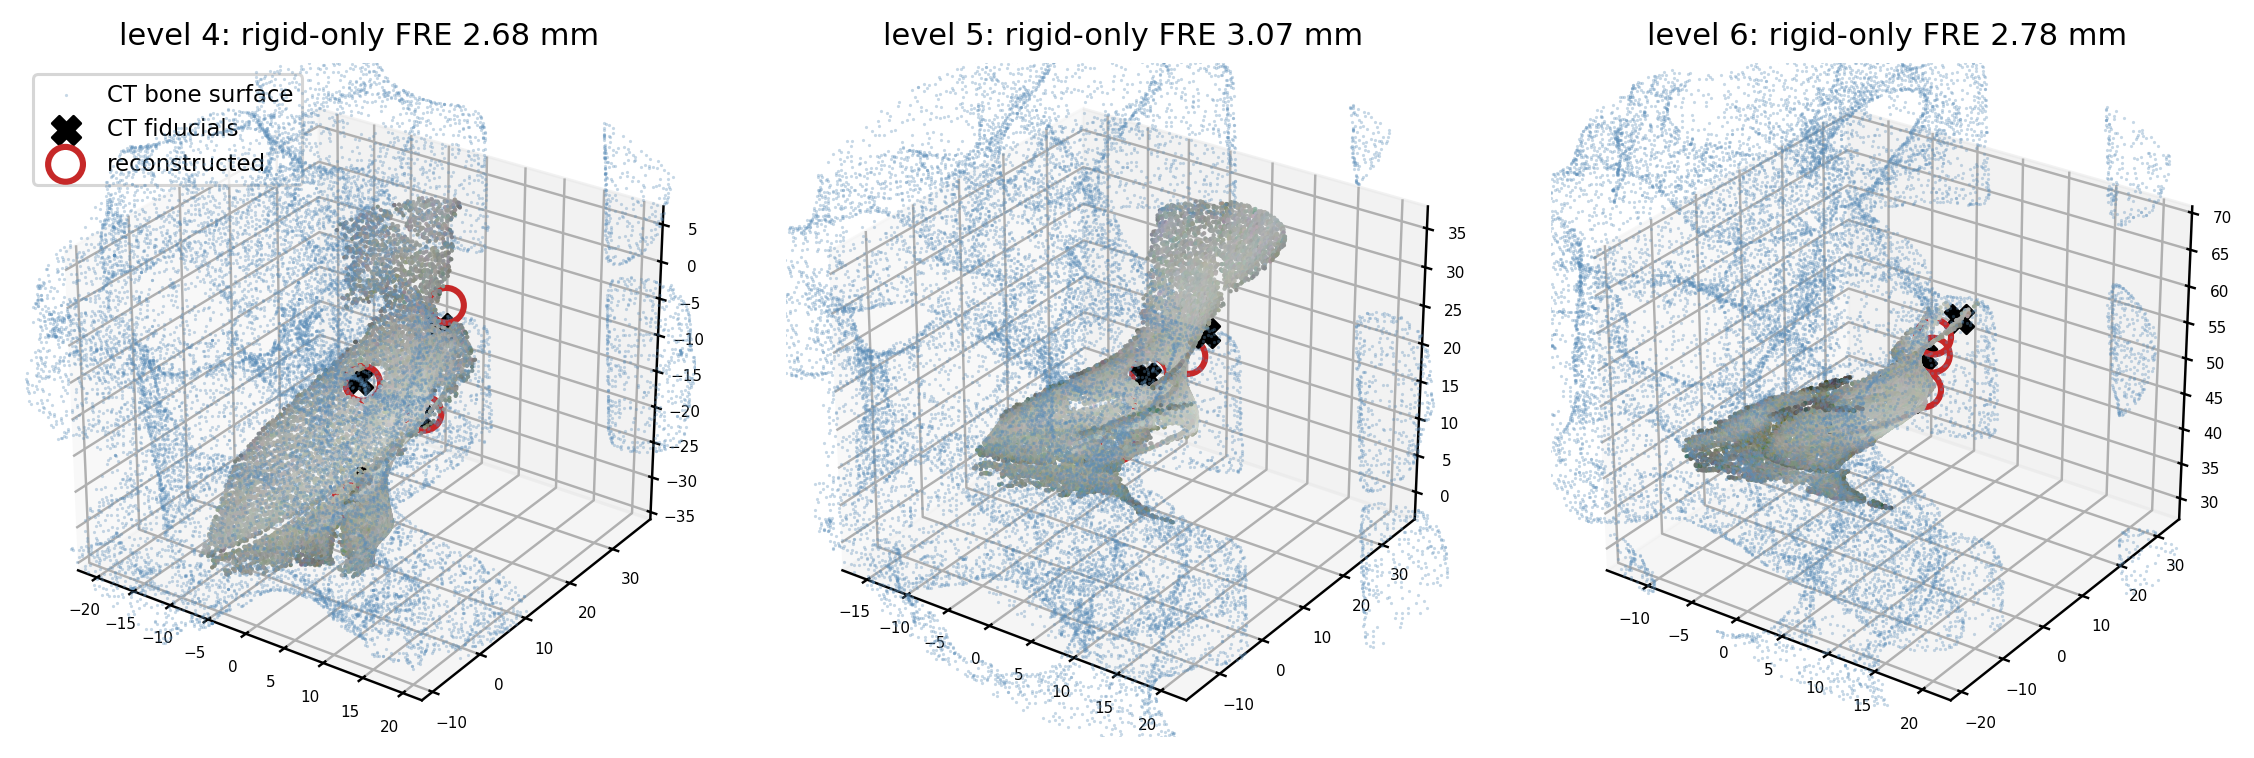
\includegraphics[width=0.92\textwidth]{figures/fig_overlay.png}
\caption{Reconstructed surfaces of the three well-conditioned levels in
CT coordinates after a rigid 6-DOF alignment (no scale correction).
Open circles: reconstructed fiducials; crosses: ground truth.  The
residual mismatch is dominated by the scale error of the solve
(Sec.~\ref{sub:main}), which the 6-DOF alignment does not absorb.}
\label{fig:overlay}
\end{figure*}

\subsection{What the Residual Does and Does Not Select}\label{sub:landscape}
Fig.~\ref{fig:landscape} shows the flat-plane residual landscape
$E(b,1;\mu)$ and a convergence trace.  The landscape is informative but
shallow, with a $(b,\mu)$ trade-off valley---fixing $\mu^\ast$ removes
this degeneracy, and the focus band removes the false close-and-flat
basin that remains.  On level~4 that removal is literal: the descent is
stopped by the band's lower edge rather than by an interior minimum
(Fig.~\ref{fig:landscape}b), so there the prior, not the residual, sets
$b$; level~5 stops within \SI{0.55}{\milli\meter} of the same edge.

\begin{figure}[t]
\centering
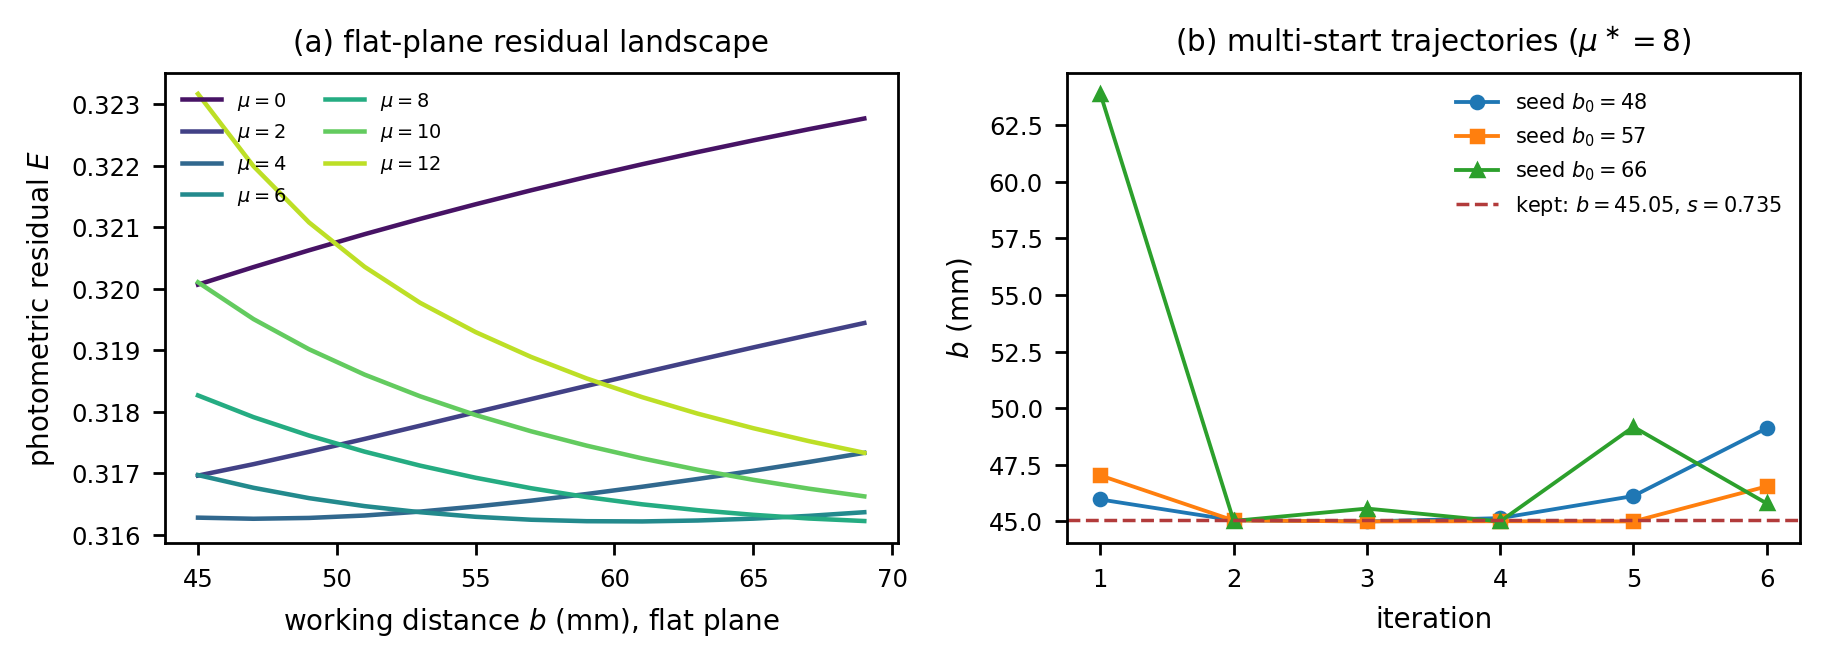
\includegraphics[width=\columnwidth]{figures/fig_landscape.png}
\caption{Level 4.  (a)~Flat-plane photometric residual vs.\ working
distance $b$ for each candidate emission exponent $\mu$: the total
variation across the focus band is ${<}2.5\%$---informative but shallow,
and nearly $\mu$-degenerate, motivating the focus-band prior and the
pinned rig-level $\mu^\ast$.  (b)~Working-distance traces of
Alg.~\ref{alg:metric} from the three seeds; all descend to
$b\approx\SI{45}{\milli\meter}$, and the photometrically best iterate
(dashed) is kept.}
\label{fig:landscape}
\end{figure}

\subsection{Baselines}\label{sub:baselines}
\textbf{Far-field.}  The far-field solve integrates its geometric mis-fit
into a low-frequency bowl (Fig.~\ref{fig:bowl}); even with depth
anchoring it reaches millimetre FRE only where the surface happens to be
benign (levels~4--5) and fails structurally on level~6
(\SI{6.57}{\milli\meter}), which the near-field model repairs
(\SI{1.74}{\milli\meter}).  \textbf{Inverse-square.}  Estimating range
directly from brightness (range $\propto I^{-1/2}$) with identical
anchoring fails on every level---\SIrange{6.4}{9.6}{\milli\meter} FRE and
grossly inflated relief---because it conflates albedo with range on
textured bone; the albedo-invariant normal-based solve is not optional.

\begin{figure}[t]
\centering
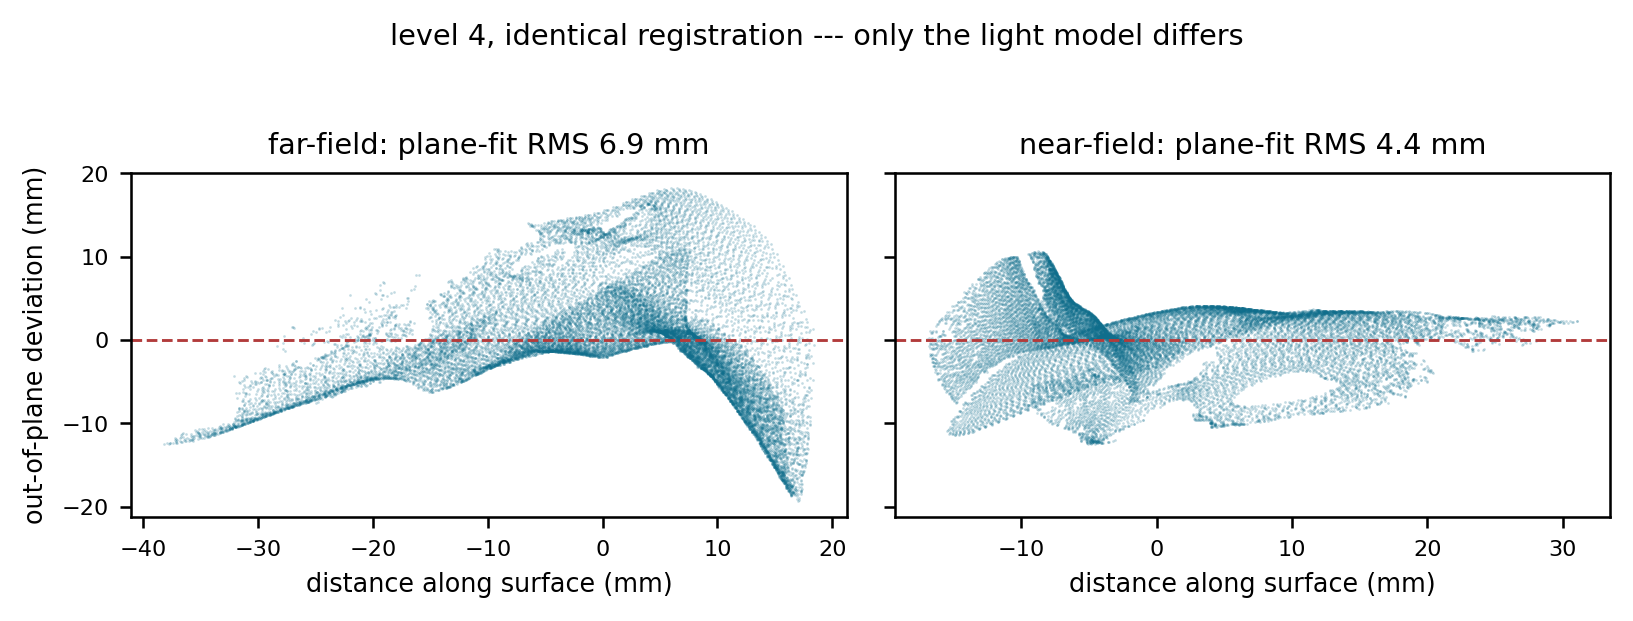
\includegraphics[width=\columnwidth]{figures/fig_bowl_new.png}
\caption{Level 4, identical data and registration, only the light model
differs: out-of-plane profiles of the reconstructed surface.  The
far-field solve (left) integrates a systematic bowl (plane-fit RMS
\SI{6.9}{\milli\meter}); the near-field solve (right) flattens it
(\SI{4.4}{\milli\meter}; the remainder is genuine bone relief).}
\label{fig:bowl}
\end{figure}

\subsection{Failure Cases}\label{sub:fail}
\emph{Level~7} has three fiducials: the rigid alignment is minimally
constrained, the scale check rests on three pairwise distances, and the
recovered $b$ rails at the top of the focus band; FRE degrades to
\SI{6.02}{\milli\meter}.  The anchored protocol is itself degenerate with
three fiducials (P3P admits up to four poses), so its
\SI{9.72}{\milli\meter} is not a meaningful comparator.  \emph{Level~8}
collapses under both protocols---the near-field confidence mask empties
while the far-field solve on the same frames stays stable---an unresolved
solver-robustness issue, not a distance effect (all captures lie at
\SIrange{51}{60}{\milli\meter}).  Separately, the recovered $b$ sits at
or within \SI{0.6}{\milli\meter} of a band edge on levels~4, 5, and~7
(0.05, 0.55, and \SI{0.11}{\milli\meter} respectively), indicating that
the $b$-gradient of $E$ is weak at this $\alpha$; band-edge convergence
is therefore a useful per-capture self-diagnostic.

\subsection{Accuracy in Context}\label{sub:context}
Table~\ref{tab:context} situates the result; metrics and conditions
differ across rows.  Three readings emerge.  First, \SIrange{2.7}{3.1}{\milli\meter} from a single
pose of a four-LED scope is inside the accuracy class of the best
calibrated near-field photometric stereo on a lab rig with 52 LEDs at
10--30 cm (\SI{3.2}{\milli\meter} mean depth error~\cite{mecca2021luces})
and of multi-view neural reconstruction given ground-truth-registered
poses (\SI{2.80}{\milli\meter}~\cite{batlle2023lightneus})---obtained
here with no pose input, no parallax, no learning, and scale from a
\SI{6.05}{\milli\meter} baseline at \SI{55}{\milli\meter}.  The
\SIrange{10}{21}{\percent} scale errors are likewise in class:
EndoMetric, the comparable illumination-baseline system evaluated on
real scenes, deviates \SI{13}{\percent} from the endoscopist's estimate
on real polyps at a more favourable baseline-to-distance
ratio~\cite{iranzo2025endometric}.  Second, it
does not yet match contact or structured-light registration
(\SIrange{0.96}{1.2}{\milli\meter}~\cite{tamura2005,jakubovic2018}) or
deployed navigation (1.2--1.75 mm~\cite{guha2017})---though the
structured-light system's clinical 95th-percentile errors reach
\SIrange{3.4}{4.3}{\milli\meter}~\cite{jakubovic2018}; the oracle-anchored
bound (\SIrange{1.32}{1.74}{\milli\meter}) shows that the photometric
solve supports that class when depth is externally anchored; recovering
it without the anchor is what bench LED calibration targets.  Third, the operating point differs in kind: those systems need an open
exposure or line of sight, which the corridors that motivate this
work---tubular retractors, arthroscopic portals, endonasal
approaches---do not offer; and navigation accuracy silently erodes
intraoperatively---manipulation, respiration, and distance from the
reference frame each contribute millimetres~\cite{guha2019}---while a
sensor inside the corridor could re-register on demand without
re-imaging.  That, not raw accuracy, is the niche this class of system
targets.

\begin{table}[t]\centering
\caption{Reported accuracy of related systems.  Metrics and conditions
differ (RMS vs.\ MAE; phantom vs.\ clinical); the table situates, it does
not rank.}
\label{tab:context}\footnotesize
\setlength{\tabcolsep}{2.8pt}
\begin{tabular}{lll}
\toprule
Method & Evaluation & Error (mm)\\
\midrule
\textbf{Ours} (1 pose, 4 LEDs, \SI{55}{\milli\meter}) & phantom, CT fid. & 2.68--3.07\\
\ \ + oracle depth anchor & phantom, CT fid. & 1.32--1.74\\
Tracked stylus, 20 pts~\cite{tamura2005} & dry-bone phantom & 0.96 RMS\\
Structured light~\cite{jakubovic2018} & clinical screws & ${\sim}$1.2 med.\\
3-D navigation~\cite{guha2017} & clinical screws & 1.2--1.75\\
LightNeuS, 20 views + poses~\cite{batlle2023lightneus} & colon phantom & 2.80 MAE\\
Single-view near-light~\cite{batlle2022photometric} & simulation & 2.8 (7\%)\\
LightDepth, scale-aligned~\cite{rodriguezpuigvert2023lightdepth} & colon phantom & 3.7--4.4 MAE\\
Near-field PS, 52 LEDs~\cite{mecca2021luces} & lab objects & 3.17 depth\\
\bottomrule
\end{tabular}
\end{table}

\subsection{Discussion and Limitations}\label{sub:lim}
The dominant residual is the assumed LED geometry: positions on an ideal
coplanar ring and a symmetric $\cos^{\mu^\ast}$ emission, both
contradicted in detail by the as-built hardware---the measured
${\sim}\SI{2}{\milli\meter}$ axial emitter spread (Sec.~\ref{sub:hw}) and
the convergent aim (Sec.~\ref{sub:wiring}).  Bench calibration of per-LED
position, aim, and
profile~\cite{queau2018led,ma2023robust,park2014nonisotropic} is the
clear next step and should tighten both scale and $b$.  The focus band is
a weak prior in principle, but it is a lens property, measurable once on
the bench.  Validation covers a single anatomy---the posterior elements of one
rigid lumbar foam phantom---whose reflectance differs from wet bone
(subsurface scatter, blood, and instrument clutter are untested);
articular and skull-base bone differ again in reflectance, moisture, and
working distance, so extension to those corridors remains to be
demonstrated.  Per-level fiducial counts limit the statistical strength
of each FRE.  Runtime (minutes per capture, unoptimised Python) is
compatible with a registration step, not with live video.

%=======================================================================
\section{CONCLUSIONS}
A near-coaxial four-LED endoscope can measure exposed bone metrically
from a single pose: tying candidate normals to a two-parameter depth
family turns the redundancy of the four-light solve into a selector for
working distance and relief gain, with the LED ring baseline providing
absolute scale and a bench focus band as the only prior.  On a
CT-instrumented lumbar spine phantom the method reaches
\SIrange{2.7}{3.1}{\milli\meter} rigid-only fiducial RMS on every
well-conditioned level---within a factor 1.6--2.3 of an oracle-anchored
bound---where far-field photometric stereo suffers a structural bowl and
inverse-square ranging fails outright.  Bench LED calibration to close
the oracle gap, a working-distance sweep, and additional specimens are
the direct next steps toward in-corridor registration---per vertebra in
the spine, and beyond it wherever bone meets a narrow approach---from
the scope already in the field, with no added radiation.

%=======================================================================
\bibliographystyle{IEEEtran}
\bibliography{luminabone}

\end{document}
